\documentclass[twocolumn]{article}

\usepackage{graphicx}
\usepackage{amsmath}
\usepackage{amsthm}
\usepackage{amssymb}
\usepackage{url}
\usepackage{multirow}
\usepackage{times}
\usepackage{fullpage}

\newcommand{\comment}[1]{}

\title{CS315: Group 08 \\
Personal Schedular}
\author{
\begin{tabular}{ccc}
	Mohit Kumar Garg & Prithvi Sharma & Sahil Solanki \\
	11431 & 11541 & 11624 \\
	\url{mohitkg@iitk.ac.in} & \url{prithvis@iitk.ac.in} & \url{ssolanki@iitk.ac.in} \\
	Dept. of CSE & Dept. of CSE & Dept. of CSE \\
	\multicolumn{3}{c}{Indian Institute of Technology, Kanpur}
\end{tabular}
}
\date{Final report \\	% replace by ``initial'' or ``final'' as appropriate
12th April, 2014}	% replace by actual date of submission or \today

\begin{document}

\maketitle

\begin{abstract}
	%
	\emph{
	For a quarter of a century, the relational database (RDBMS) has been the dominant model for database management. 	But, today, non-relational ``NoSQL" databases are gaining mindshare as an alternative model for database management. This project was undertaken to develop a practical understanding of the basics of NoSQL, particulary mongoDB, by creating a simple web application \textbf{`Personal Schedular'}.}\\ 
	%
\end{abstract}

\section{Introduction and Problem Statement}
The problem statement is to get acquainted with the MongoDB framework and create a scheduler application in the process. \newline \newline
We have created a web application aimed at university students and professors. The scheduler allows the users to list out their regular academic and personal schedules in a structured way with some other added functionalities. This will be helpful for effective time management. The academic schedule of a student is determind in the beginning of the semester and remain same for the whole semester. In order to avoid adding the repeatative schedule of classes every week, a student can mention the courses he/she is attending and they will be automaticly added in their schedule for the whole semester. \newline
Sometimes an instructor needs to take extra classes apart from the regular classes and generally it becomes a headache for the instructor to come up with a time which is condusive for all the students. Having this motivation in mind, we develp this application to provide an efficient tool for the instructor so that he need not to waste the valuable class hours in discussing the timing of extra class. \\     




\subsection{Related Material}

\textbf{Technologies used:-} MongoDB, HTML, CSS, JavaScript, jQuery
\newline
\textbf{Frameworks and Libraries used:-} Twitter Bootstrap, Arshaw FullCalendar jQuery plugin, PHP Driver for MongoDB
\comment{

Can also comment out paragraphs, etc.

}
\section{Database Description}
In this application we maintain 4 collections. 

\begin{enumerate}
  \item \textbf{Users} : This is to keep the details of all the registered users like username, password, list of courses.
  \item \textbf{Courses} : This to keep the details of the courses that are currently offered. This stores course name, instructor name, day and timing of class, students registered in that course, scheduled extra classes. Instructor can add a course in this collection.
  \item \textbf{Personal Schedule} : For every user this stores the non-academic activities. A user can add an activity with date, time and description.

\end{enumerate}

\section{Algorithm or Approach}
%In order to keep 
\begin{enumerate}
\item \textbf{Populate the activities in the calendar} : For a user iterate through all the courses he/she is taking, for each course query the regular and extra-class scheudule from \emph{Courses} and populate it in the calendar. Then query the personal schedule from \emph{Personal Schedule} and populate this too.  
\item \textbf{Scheduling Extra Class} : Let say the instructor wants to schedule an extra class of course \textbf{c}. \emph{student-list(c)} is the list of students taking the course c. Let \emph{CoursesUnion(c)} be the union of all the courses taken by the users in student-list(c). Now iterate through \emph{CoursesUnion(c)}  and check if that course has any reular/extra class on the time specified by instructor.\\

\end{enumerate}

%We maintain two collections. One for keeping the schedule of every person and other to keep the details of the courses. A student can add the schedule of the course in his personal schedule by joining that course.
%A user can have two type of activities in his daily schedule, one which are repeative in nature e.g. class of CS315 on every Tuesday and Friday, and other which are not repeatative (or less frequent) e.g. appointment with dentist.\\
%the collection of \emph{courses} keeps the list of students enrolled in a courses. So when an instructor query to arrange an extra class, the code iteratively check every student and list all the students who have any academic activity scheduled at that time slot. If there is no such student then it is a fruitful situation for instructor. And when the instructor schedules an extra class then it will notify all the students registered in the course.

%Details of the method.
%Put in a pseudo-code, etc. if applicable.
%Explain with figures.
%This application was aimed to serve as both a	 personal schedular as well as academics schedular




Use the following format for figures:

\begin{figure}[t]
	\centering
	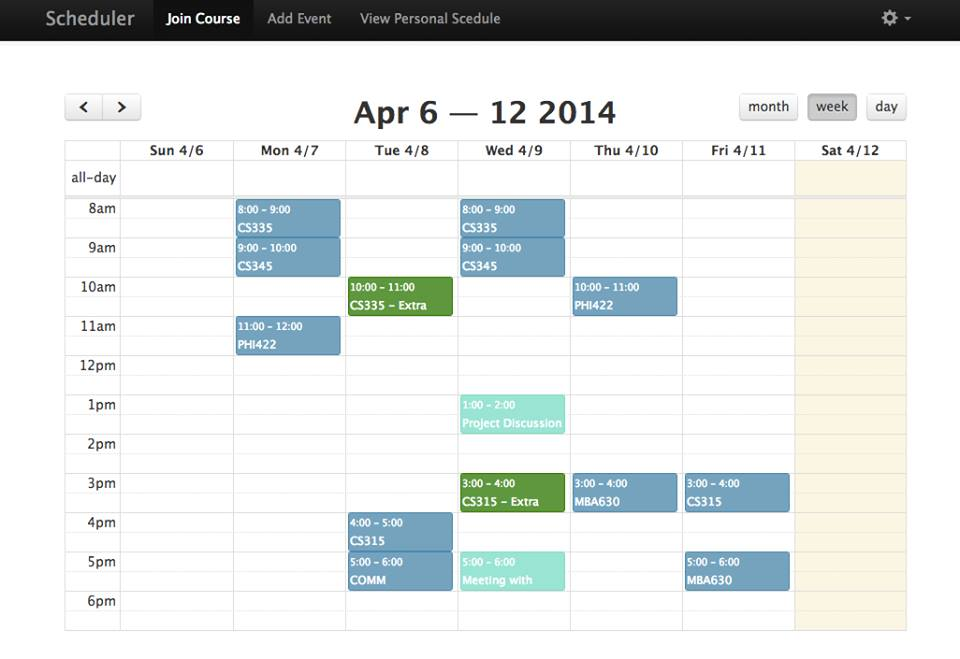
\includegraphics[width=80mm]{week.jpg}
	\caption{Weekly Schedule}
	\label{weekly schedule}
\end{figure}

\begin{figure}[t]
	\centering
	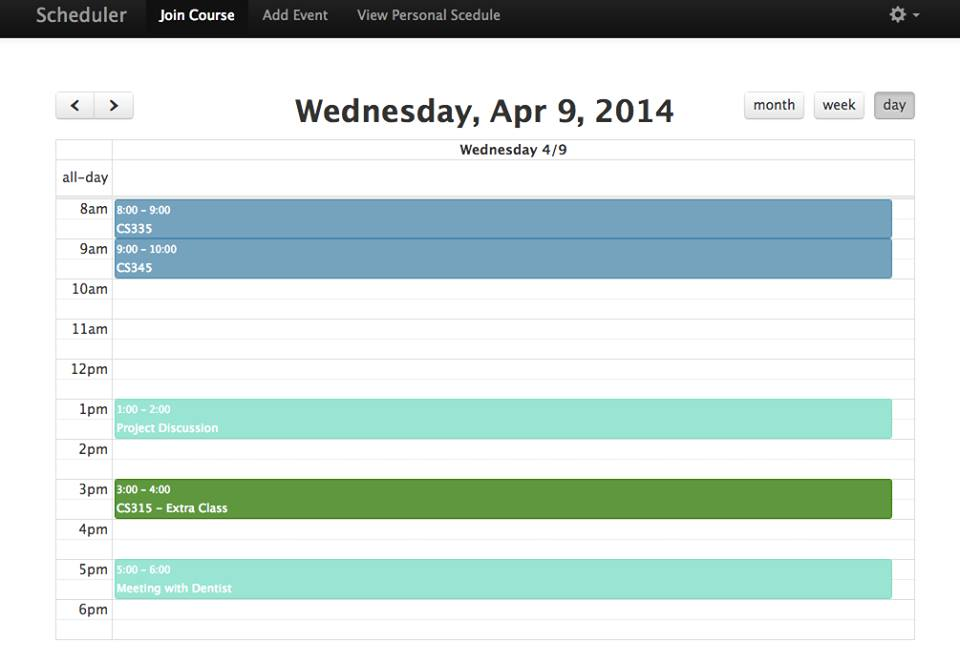
\includegraphics[width=80mm]{day.jpg}
	\caption{Daily Schedule}
	\label{weekly schedule}
\end{figure}



\section{Results}

Details of results, in tabular and/or graphical formats.

More importantly, analyze the results.

\comment{

\begin{table}[t]
	\centering
	\begin{tabular}{|c||cc|}
		\hline
		Header 1 & Desc 1 & Desc 2 \\
		\hline
		\hline
		Row 1 & Data 1-1 & Data 1-2 \\
		Row 2 & Data 2-1 & Data 2-2 \\
		\hline
	\end{tabular}
	\caption{Table of results.}
	\label{tab:results}
\end{table}

And refer as Table \ref{tab:results}.

}

\section{Conclusions}
During the course of development of the web application, following properties of MongoDB were observed:
\subsection*{Positives}
\begin{enumerate}
\item \textbf{Schemaless} - As MongoDB is a document data store, it is schemaless in nature and thus it is extremely easy to add new fields or completely change the structure of a model. 
\item \textbf{Query Language} - Querying into documents is very easy due to the JSON document storage model. Features can be built quickly with advanced queries.
\item \textbf{Fully-featured Drivers} - Official MongoDB drivers are available for all major industry languages.
\end{enumerate} 

\subsection*{Negatives} 
Specific to our relatively simple project, there is nothing in which MongoDB lacks in comparison to relational databases. \newline 
But, on further research about how MongoDB databases are implemented at the lowest level, we found some issues people have faced with MongoDB of which a prominent one is the following:-
\begin{enumerate}
\item \textbf{Uncompressed field names} - MongoDB supports arbitrary documents in a collection. Now, because most of the field names are similar, if one stores 1000 documents with the key "name", "name" is stored 1000 times in the data set instead of shortening the field name or linking all same key names to a location which seems an overkill.
\end{enumerate}

%\section*{References}
%
%Directly type in bib entries.
%
%Better is to use bibtex.
\begin{thebibliography}{9}


\bibitem{mongoGuide}http://docs.mongodb.org/manual/

\bibitem{Canlendar}
http://arshaw.com/fullcalendar/

\bibitem{bootstrap} http://getbootstrap.com/


\end{thebibliography}

\end{document}
